\documentclass{article}
\usepackage{graphicx}
\usepackage{tikz}
\usepackage{amsmath}
\usepackage{hyperref}
\title{Page Ranking Algorithm}

\author{
    Armen Ghazaryan \\
    \textit{American University of Armenia} \\
    \texttt{armen.ghazaryan004@gmail.com}
    \and
    Kima Badalyan \\
    \textit{American University of Armenia} \\
    \texttt{kimabadalyan4004@gmail.com}
    \and
    Melani Melkonyan \\
    \textit{American University of Armenia} \\
    \texttt{melani\_melkonyan@edu.aua.am}
}

\date{} % This removes the date

\begin{document}
\maketitle

\begin{abstract}
In today's digital age, managing and navigating the vast expanse of information available on the internet poses significant challenges. Search engines use complex algorithms to organize and prioritize web content to address this issue. The Google PageRank algorithm is a fundamental tool for ranking web pages in search engine results. This paper presents a comprehensive study of the PageRank algorithm, focusing on its mathematical foundation and numerical implementation. We begin by explaining the algorithm's basic principles highlighting its reliance on the concept of eigenvectors and eigenvalues. Next, we delve into the mathematical formulation of the algorithm, detailing the iterative steps used to calculate the PageRank scores. We demonstrate how these steps can be implemented computationally through numerical methods such as the power method. Additionally, we discuss the practical aspects of implementing the algorithm in Python, including web scraping techniques to gather relevant data. Finally, we present our findings and insights into the inner workings of the PageRank algorithm, showcasing its effectiveness in ranking web pages based on their importance and relevance.
\end{abstract}

\section{Introduction}
The PageRank algorithm's effectiveness lies in its ability to model the web as a graph, with web pages represented as nodes and hyperlinks as edges. Through iterative computation, PageRank assigns a numerical score to each web page, reflecting its relative importance within the web graph. This score is influenced not only by the number of incoming links but also by the quality and relevance of those links, thereby providing a measure of a page's significance.

In the late 1990s, the web search landscape was undergoing a profound transformation. Traditional search engines relied solely on textual content to rank pages, but a groundbreaking model emerged, promising more effective results by analyzing the web's hyperlink structure. Sergey Brin and Larry Page, then doctoral candidates at Stanford University, were refining PageRank, their innovative approach to web search. In 1998, Brin and Page temporarily left Stanford to focus on their startup, Google, which was rapidly gaining attention for its novel search algorithm. In a paper presented at WWW98, they outlined the anatomy of their hypertextual search engine, setting the stage for PageRank's ascension. PageRank, with its query independence and resilience to spam, ultimately became the dominant model, leading Google to unprecedented success. This period marked a crucial moment in search engine history.

In the subsequent sections of this paper, we will outline the methodology used in our project, discuss the results obtained, and analyze the implications of our findings.

\section{Mathematical Solution of Google PageRank Algorithm}

Let us consider that we have 8 web pages, and we want to find the Google PageRank of each web page. We will have a graph representing the connections between these 8 websites, where the arrows represent the links, taking the linking website as the starting point and the linked website as the ending point.

\begin{figure}[htbp]
    \centering
    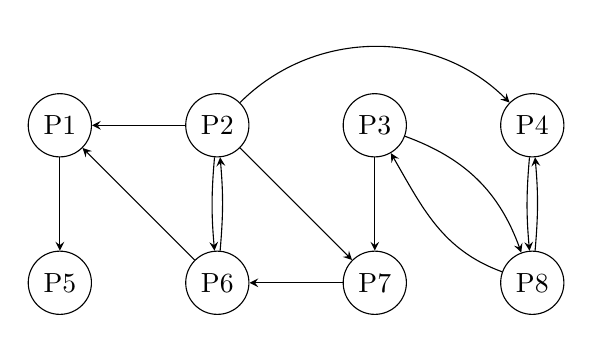
\begin{tikzpicture}[>=stealth, every node/.style={circle, draw}]
      % First row of nodes
      \node (P1) at (0,0) {P1};
      \node (P2) at (2,0) {P2};
      \node (P3) at (4,0) {P3};
      \node (P4) at (6,0) {P4};
      
      % Second row of nodes
      \node (P5) at (0,-2) {P5};
      \node (P6) at (2,-2) {P6};
      \node (P7) at (4,-2) {P7};
      \node (P8) at (6,-2) {P8};
      
      % Arrows
      \draw[->] (P1) -- (P5);
      \draw[->] (P2) -- (P1);
      \draw[->] (P2) to[out=-95,in=95](P6);
      \draw[->] (P6) to[out=85,in=-85](P2);
      \draw[->] (P2) -- (P7);
      \draw[->] (P3) -- (P7);
      \draw[->] (P3) to[out=-20,in=110] (P8);
      \draw[->] (P8) to[out=-200,in=-60] (P3);
      \draw[->] (P4) to[out=-95,in=95](P8);
      \draw[->] (P8) to[out=85,in=-85](P4);
      \draw[->] (P6) -- (P1);
      \draw[->] (P7) -- (P6);
      \draw[->] (P2) to[out=45,in=135] (P4); % Arrow from P2 to P4
    \end{tikzpicture}
    \caption{Graph representing the connections between 8 web pages.}
    \label{fig:web_graph}
\end{figure}

We can construct the relationship matrix \( A \) of these 8 webpages and call it a hyperlink matrix, where we have 1s in \( A_{i,j} \) entry if there is a hyperlink from \( P_i \) to \( P_j \) and 0 otherwise.

\[ A = \begin{bmatrix}
0 & 0 & 0 & 0 & 1 & 0 & 0 & 0 \\
1 & 0 & 0 & 1 & 0 & 1 & 1 & 0 \\
0 & 0 & 0 & 0 & 0 & 0 & 1 & 1 \\
0 & 0 & 0 & 0 & 0 & 0 & 0 & 1 \\
0 & 0 & 0 & 0 & 0 & 0 & 0 & 0 \\
1 & 1 & 0 & 0 & 0 & 0 & 0 & 0 \\
0 & 0 & 0 & 0 & 0 & 1 & 0 & 0 \\
0 & 0 & 1 & 1 & 0 & 0 & 0 & 0 \\
\end{bmatrix} \]

For now, let’s understand what PageRank is and how it is calculated. PageRank is the measure of the importance of a web. The PageRank of one webpage is calculated using the number of all the hyperlinks to that webpage. However, it is not only about how many hyperlinks are to the linked webpage but also the number of hyperlinks the linking webpage links to other web pages. To make it more understandable, let’s consider this real-life example. Artists receive various awards every year from different organizations. However, some organization’s awards are more valuable than others because not every artist can receive an award from them, while other organizations award every other individual in the industry.

Consider that we have a hyperlink \( P_j \to P_i \). 
Let’s denote the PageRank of \( P_i \) by \( r(P_i) \) and the number of outlinks of \( P_i \) denote by \( |P_i| \).
The value of the hyperlink from \( P_j \) will be equal to 

\[ \frac{r(P_j)}{|P_j|} \]

The PageRank of each \( P_i \) will be equal to the sum of the values of all the hyperlinks to \( P_i \).

\[ r(P_i) = \sum \left( \frac{r(P_j)}{|P_j|} \right) \]
\\

We can now construct a system calculating the PageRank of each of our 8 web pages.


\[
\begin{cases}
r(P_1) &= \frac{r(P_2)}{4} + \frac{r(P_6)}{2} \\
r(P_2) &= \frac{r(P_6)}{2} \\
r(P_3) &= \frac{r(P_8)}{2} \\
r(P_4) &= \frac{r(P_8)}{2} + \frac{r(P_2)}{4} \\
r(P_5) &= r(P_1) \\
r(P_6) &= \frac{r(P_2)}{4} + r(P_7) \\
r(P_7) &= \frac{r(P_2)}{4} + \frac{r(P_3)}{2} \\
r(P_8) &= \frac{r(P_3)}{2} + r(P_4) \\
\end{cases}
\]
\\

Let’s construct the PageRank raw vector, 
\[
v = (\text{r}(P_1), \text{r}(P_2), \text{r}(P_3), \text{r}(P_4), \text{r}(P_5), \\
\begin{aligned}
 & \text{r}(P_6), \text{r}(P_7), \text{r}(P_8))
\end{aligned}
\] 
such that it satisfies the above system. Now we have 8 unknowns, \( \text{r}(P_i) \), \( i = 1, \ldots, 8 \), and we will need to solve this SLE in order to find the PageRanks of each of the web pages.


First of all, we will need to use the normalized form of our matrix \( A \). For that, we will divide each entry \( P_{i,j} \) of \( A \) by the sum of the entries of \( i \)-th row of \( A \).

\[
H = \begin{bmatrix}
0 & 0 & 0 & 0 & 1 & 0 & 0 & 0 \\
\frac{1}{4} & 0 & 0 & \frac{1}{4} & 0 & \frac{1}{4} & \frac{1}{4} & 0 \\
0 & 0 & 0 & 0 & 0 & 0 & \frac{1}{2} & \frac{1}{2} \\
0 & 0 & 0 & 0 & 0 & 0 & 0 & 1 \\
0 & 0 & 0 & 0 & 0 & 0 & 0 & 0 \\
\frac{1}{2} & \frac{1}{2} & 0 & 0 & 0 & 0 & 0 & 0 \\
0 & 0 & 0 & 0 & 0 & 1 & 0 & 0 \\
0 & 0 & \frac{1}{2} & \frac{1}{2} & 0 & 0 & 0 & 0 \\
\end{bmatrix}
\]
\\

In order to find our final \( v \), we will need to construct a sequence \( v_n \), which will finally converge to our \( v \). For that, we will introduce the new mathematical concept, which is the direct iteration method for finding the dominant eigenvector of our matrix \( H \), called the power method.
\\ 

The power method starts with an initial guess for the dominant eigenvector (often an equally weighted vector representing the probability of being on any particular page, which is the same for every page). Every next approximation is calculated by using the formula below.

\[ v^{(k+1)} = v^{(k)} H \]

After several iterations, the result should converge to our desired dominant eigenvector, which is also a probability vector. The final vector \( v \) will eventually show the page rank of each website (nodes of the graph in our case).
\\

Before finding the dominant eigenvector \( v \), we need to answer these important questions:
\\

\begin{itemize}
    \item[1.] Under what circumstances or properties of \( H \) is it guaranteed to converge?
    \item[2.] Does convergence depend on the initial vector?
    \item[3.] And if it converges, is the \( v \) vector to which it converges necessarily a probability vector?
\end{itemize}

To address the first question, let us first implement the power method on \( H \) and use the following as an initial vector: 
\[ v^{(0)} = \left( \frac{1}{8}, \frac{1}{8}, \frac{1}{8}, \frac{1}{8}, \frac{1}{8}, \frac{1}{8}, \frac{1}{8}, \frac{1}{8} \right) \]

Then, iteratively calculate \( v^{(1)} \), \( v^{(2)} \), ..., \( v^{(n)} \), which, you can see below, doesn't converge to a probability vector, as its entries don’t sum up to 1.

\begin{verbatim}
print(v)
# Output: [0.00326713 0.00248645 0.00582769 0.00660836 0.00388064 
# 0.00510539 0.00345665 0.00878588]

sum(v)
# Output: 0.03941818710023881
\end{verbatim}
\\

This problem is caused by zero rows of the \( H \) matrix. The row containing zeros indicates that \( P5 \) is a dangling node, meaning it has no outgoing links. Real-life examples of dangling nodes can be PDF documents with no outlinks, and when entering a dangling node, a web surfer is stuck in it, as there's no way to leave the node.

To overcome this problem, Brin and Page declared that whenever a web surfer enters a dangling node, he jumps to any page randomly. From a mathematical point of view, this means replacing zero rows of the \( H \) matrix with rows of \( \frac{1}{n} \)'s, where \( n \) is the number of all nodes in our graph. Let us denote our new matrix as \( S \):

\[
S = \begin{bmatrix}
0 & 0 & 0 & 0 & 1 & 0 & 0 & 0 \\
\frac{1}{4} & 0 & 0 & \frac{1}{4} & 0 & \frac{1}{4} & \frac{1}{4} & 0 \\
0 & 0 & 0 & 0 & 0 & 0 & \frac{1}{2} & \frac{1}{2} \\
0 & 0 & 0 & 0 & 0 & 0 & 0 & 1 \\
\frac{1}{8} & \frac{1}{8} & \frac{1}{8} & \frac{1}{8} & \frac{1}{8} & \frac{1}{8} & \frac{1}{8} & \frac{1}{8} \\
\frac{1}{2} & \frac{1}{2} & 0 & 0 & 0 & 0 & 0 & 0 \\
0 & 0 & 0 & 0 & 0 & 1 & 0 & 0 \\
0 & 0 & \frac{1}{2} & \frac{1}{2} & 0 & 0 & 0 & 0 \\
\end{bmatrix}
\]
\\

The obtained new matrix is a stochastic matrix, as the sum of each row's elements is 1. As the matrix is stochastic, it is the transition probability matrix for a Markov chain. Recalling the notion of the Markov chain and logic of random walk in the Google PageRank algorithm both state that a web surfer's next visit does not depend on the pages that it visited in the past — that choice depends only on the current page.
\\

To answer the second and the third questions, we can see that in this stage of the algorithm using the power method applied to the matrix \( S \), the notion of the Markov chain ensures that for any starting vector, the \( v_n \) sequence converges to a unique positive vector as long as \( S \) is stochastic, irreducible, and aperiodic.
\\

After these changes, let us perform the same power method, but now, we are using \( S \) instead of \( H \):

\[ v(k+1) = v(k)S \]

As you can see from the result, now our sequence converges to the following vector, which, in fact, is a probability vector:

\begin{verbatim}
print(v)
# Output: [0.0982008  0.07849338 0.12400246 0.14370988 0.11247178 
# 0.12946709 0.09530559 0.21834903]

sum(v)
# Output: 1
\end{verbatim}


From this, we can conclude that by introducing the Stochastic matrix \( S \), we solve the problem of dangling nodes and ensure that the final vector \( v \) exists and will be a probability vector.
\\

However, there is another problem we have to consider: Are all the elements of our probability vector positive, i.e., is the \( v \) vector a positive vector? As mentioned above, the positivity of a probability vector depends on a matrix being stochastic, irreducible, and aperiodic. We've already turned our matrix into a stochastic matrix. So what about being irreducible and aperiodic? For this, we need to make some adjustments to our matrix \( S \).
\\


This is when we introduce a new concept - the damping factor. This factor describes the behavior of random walking, where from time to time, when a web surfer becomes bored, it easily can request a random webpage. The proportion of time when it continues to follow links is \( d \), and \( 1-d \) is the proportion of time when it randomly changes to another webpage (\( d \in (0, 1) \)). This will result in the modification for each row \( r \):

\[ dr+(1-d)\left(\frac{1}{8}, \frac{1}{8}, \frac{1}{8}, \frac{1}{8}, \frac{1}{8}, \frac{1}{8}, \frac{1}{8}, \frac{1}{8}\right) \]
\\


This results in the whole matrix's change:

\[ G=dS + (1-d)J\]

where \( J \) is the following matrix:

\[ \mathbf{J} = \begin{bmatrix}
\frac{1}{8} & \frac{1}{8} & \frac{1}{8} & \frac{1}{8} & \frac{1}{8} & \frac{1}{8} & \frac{1}{8} & \frac{1}{8} \\
\frac{1}{8} & \frac{1}{8} & \frac{1}{8} & \frac{1}{8} & \frac{1}{8} & \frac{1}{8} & \frac{1}{8} & \frac{1}{8} \\
\frac{1}{8} & \frac{1}{8} & \frac{1}{8} & \frac{1}{8} & \frac{1}{8} & \frac{1}{8} & \frac{1}{8} & \frac{1}{8} \\
\frac{1}{8} & \frac{1}{8} & \frac{1}{8} & \frac{1}{8} & \frac{1}{8} & \frac{1}{8} & \frac{1}{8} & \frac{1}{8} \\
\frac{1}{8} & \frac{1}{8} & \frac{1}{8} & \frac{1}{8} & \frac{1}{8} & \frac{1}{8} & \frac{1}{8} & \frac{1}{8} \\
\frac{1}{8} & \frac{1}{8} & \frac{1}{8} & \frac{1}{8} & \frac{1}{8} & \frac{1}{8} & \frac{1}{8} & \frac{1}{8} \\
\frac{1}{8} & \frac{1}{8} & \frac{1}{8} & \frac{1}{8} & \frac{1}{8} & \frac{1}{8} & \frac{1}{8} & \frac{1}{8} \\
\frac{1}{8} & \frac{1}{8} & \frac{1}{8} & \frac{1}{8} & \frac{1}{8} & \frac{1}{8} & \frac{1}{8} & \frac{1}{8} \\
\end{bmatrix} \]
\\

\begin{itemize}
    \item \( G \) is irreducible. Every page is directly connected to every other page, so irreducibility is enforced.
    \item \( G \) is aperiodic. The self-loops (\( G_{ii} > 0 \) for all \( i \)) create aperiodicity.
\end{itemize}

\( G \) is our new modified matrix, which is also called the Google Matrix. In their original paper written in 1998, \( d = 0.85 \), which is considered the usual measure of \( d \) in Google. 
These modifications allow us to fully use the notion of the Markov chain, as the \( G \) matrix is stochastic, aperiodic, and irreducible.
\\

Now, when we iteratively go through the equation

\[ v(k+1) = v(k)G \]
\\

Ultimately, we get that our sequence \( v_n \) surely converges to \( v \) no matter what the initial vector \( v(0) \) was. Our \( v \) is a unique and positive probability vector.
\\

\begin{verbatim}
print(v)
# Output: [0.10868453 0.08963628 0.11443949 0.13348775 
# 0.12434487 0.13570959 0.09964369 0.1940538]

sum(v)  # round-off errors of python
# Output: 0.9999999999999997
\end{verbatim}


Thus, by subjecting our initial matrix \( H \) to some modifications, using the theory of Markov chain for stochastic matrices, and applying the power method to our final matrix \( G \), we get the unique positive probability vector to which our initial vector \( v \) converged. Our final \( v \) shows the PageRank of each web page.
\\

By listing them in descending order according to the Google PageRank, we get the following result:
\\

\begin{center}
\textbf{\Large{P$_8$, P$_6$, P$_4$, P$_5$, P$_3$, P$_1$, P$_7$, P$_2$}}
\end{center}

Finally, we can conclude that \textbf{P$_{8}$} has the highest page rank and will be disposed of first, while \textbf{P$_{2}$} has the lowest PageRank.
\\

\section{Implementations}

The implementations for this paper involved the implementation of the Google PageRank algorithm and testing it on a small sample of web pages. The process can be summarized into the following steps:

\subsection{Web Scraping}

\begin{itemize}
    \item \textbf{Web Scraping:} We started by collecting data from the web using Python's \texttt{BeautifulSoup 4} library. This involved scraping a website starting from a given URL and extracting the hyperlinks found on each web page.
    
    \item \textbf{Recursive Scraping:} The scraping process was implemented recursively, with a set to track visited URLs and a limit on the number of websites to avoid excessive data collection. This approach allowed us to construct a web structure by exploring a network of interlinked pages.
    
    \item \textbf{Data Storage:} The data collected from the scraping process was stored in a JSON file. This JSON file contained the web structure, including the links between different web pages.
\end{itemize}

\subsection{Data Preparation}

\begin{itemize}
    \item \textbf{Loading Data:} The JSON file with the web structure was loaded into another Python script for further processing.
    
    \item \textbf{Matrix Creation:} Based on the web structure data, a matrix was created. This matrix represented the connections between web pages in the form of an adjacency matrix, where each element indicated the presence or absence of a link between two web pages.
    
    \item \textbf{Normalization:} The matrix was normalized to account for variations in link density across web pages. This step is important for ensuring that the algorithm functions correctly and produces meaningful results.
\end{itemize}

\subsection{Algorithm Implementation}

\begin{itemize}
    \item \textbf{Algorithm Application:} The Google PageRank algorithm was applied to the normalized matrix. This involved calculating the rank of each web page based on the links it receives from other pages.
    
    \item \textbf{Convergence Check:} The algorithm was run iteratively until the rank values converged, indicating that the ranking process had reached a stable state.
    
    \item \textbf{Vector Analysis:} The resulting rank vector, representing the importance of each web page, was analyzed. As expected, the sum of the vector's components equaled 1, which confirms the correctness of the implementation.
\end{itemize}


In summary, the implementations involved scraping a web structure, preparing the data for analysis, implementing the Google PageRank algorithm, and testing it on a small sample. This process allowed us to explore the effectiveness of PageRank on a subset of web pages and verify the accuracy of our implementation.

\section{Why Google Page Ranking}

A wide variety of page ranking algorithms have been developed in the world of web search and informational retrieval, used to estimate the relevance and significance of web pages. They vary widely – from general principles based on the choice of keywords to complex algorithms considering linking patterns, user behavior, and content quality. Nevertheless, among many alternatives, we covered Google PageRank with several arguments behind it. One reason is that this particular algorithm formed the basis of contemporary search engines and outlined the most scalable and powerful search quality judgment algorithm. The algorithm determined the vectors of the search quality identification. Furthermore, PageRank is based on the concept of “importance by association,” which guides users to credible and dependable pages, thus resulting in improved search outcomes. In addition, Google’s constant drive towards innovation guarantees the dynamism of PageRank under various web conditions and various other digital transformation dynamics. Evidently, our decision to study the concepts of Google PageRank results from the system’s track record, scalability, and efficiency, as well as lasting applicability in the sector of search engines and information recovery.


\section{Conclusion}

In conclusion, the Google PageRank algorithm has revolutionized internet search by prioritizing web pages based on the quality and quantity of links. Despite challenges, it remains a fundamental aspect of Google's search engine. Its influence extends beyond search engines, impacting fields like social network analysis and academic citation. PageRank's relevance in the digital era is undeniable, shaping the way how we access and interact with online information.

Throughout our paper, we discussed the Google PageRank algorithm’s history, challenges that were overcome throughout its final development, and its superiority over other Page Rank algorithms. Our paper delved deep into crucial mathematical notions that lie under its implementation: we discussed how they were used. Moreover, we applied the discussed mathematical notions used in the Google PageRank algorithm to our own randomly created 8-node graph (which served as a representation of web pages): we constructed a transition matrix based on the link structure of the graph, initialized a probability vector, and iteratively applied the Power Method to calculate the PageRank scores for each node. From this experiment, we understood how this algorithm can actually be applied to real-world scenarios to rank web pages based on their importance and relevance.
\\

\section{Link to GitHub}

Using the link below find the implemetations for both mathematical part of this paper and for the Experimental Setup on 100 webpages.
\\

\href{https://github.com/armenghazaryann/PageRanking}{\textcolor{blue}{Implementations}}

\section{References}

\subsection{General Reference}
\begin{itemize}
    \item Amy N. Langville and Carl D. Meyer, \textit{Google’s PageRank and Beyond: The Science of Search Engine Rankings}, Princeton University Press, 2006.
\end{itemize}

\subsection{Technical References}
\begin{itemize}
    \item \url{https://shorturl.at/elxN4}
    \item \url{https://shorturl.at/jsyAI}
    \item \url{https://www.youtube.com/watch?v=VpiyOxiVmCg}
    \item \url{https://www.youtube.com/watch?v=meonLcN7LD4}
\end{itemize}






\end{document}